\documentclass[11pt]{article}

\usepackage{amsmath}
\usepackage{amsfonts}
\usepackage[margin=1in]{geometry}
\usepackage{enumitem}
\usepackage{graphicx}
\usepackage[colorlinks]{hyperref}
\usepackage{longtable}

\usepackage{helvet}
\renewcommand{\familydefault}{\sfdefault}

\setlength{\parindent}{0in}

\def\tightlist{}
\def\toprule{}
\def\bottomrule{}

\begin{document}
{\LARGE Homework 5 (Due October
14th)}\label{homework-5-due-october-14th}

{1. Gauss' Law and Cavities}\label{gauss-law-and-cavities}

A \textbf{metal} sphere of radius \(R\), carrying a charge \(+q\), is
surrounded by a thick concentric \textbf{metal} shell (inner radius
\(a\), outer radius \(b\)). The shell carries no net charge. Where
requested, please explain your reasoning.

\begin{figure}[htbp]
\centering
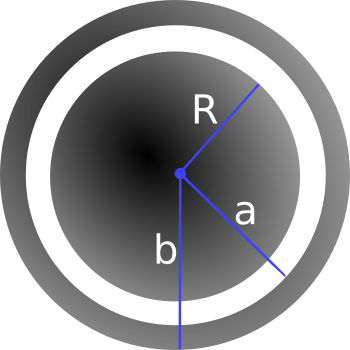
\includegraphics[width=0.5\linewidth]{./images/hw5/concentric_spheres.png}
\end{figure}

\begin{enumerate}
\def\labelenumi{\arabic{enumi}.}
\tightlist
\item
  Sketch the charge distribution everywhere. If the charge is zero
  anywhere, indicate that explicitly.
\item
  From part 1, you probably noticed the charge distributes in some way
  on the metals. Determine the surface charge density \(\sigma\) at
  \(R\), at \(a\), and at \(b\).
\item
  Sketch the electric field everywhere; explain how you know the field
  you have drawn is correct. If the field is zero anywhere, indicate
  that explicitly.
\item
  Find the potential everywhere, use \(r \rightarrow \infty\) as your
  reference point for \(V=0\).
\item
  Now the outer surface is touched by a grounding wire, which lowers its
  potential to zero. How do your answers change to parts 2 and 4?
  Explain your reasoning.
\end{enumerate}

{2. Coax capacitors}\label{coax-capacitors}

Consider a coaxial cable with an inner conducting cylinder has radius
\(a\) and the outer conducting cylindrical shell has inner radius \(b\).
It is physically easy to set up any fixed potential difference
\(\Delta V\) between the inner and outer conductors. In practice, the
cable is always electrically neutral.

\begin{enumerate}
\def\labelenumi{\arabic{enumi}.}
\tightlist
\item
  Assuming charge per length \(+\lambda\) and \(-\lambda\) on the inner
  and outer cylinders, derive a formula for the voltage difference
  \(\Delta V\) between the cylinders.
\item
  Assuming infinitely long cylinders, find the \textbf{energy stored per
  length (W/L)} inside this capacitor. \emph{Notice we are asking for
  the energy per unit length, the answer is not infinity!} Let's do it
  two ways so we can check:
\end{enumerate}

\begin{itemize}
\tightlist
\item
  Find the capacitance per length (\(C/L\)) of this system, and then use
  stored energy \(W = \frac{1}{2} C (\Delta V)^2\).
\item
  Integrate the energy density stored in the E field.
\end{itemize}

\begin{enumerate}
\def\labelenumi{\arabic{enumi}.}
\setcounter{enumi}{2}
\tightlist
\item
  Based on your answers to part 2, where in space would you say this
  energy is physically stored?
\item
  Estimate the capacitance per meter of the coaxial cable that the cable
  company uses to send TV signals into homes. Justify any assumptions.
\item
  This model is also excellent for ``axons'', which are long cylindrical
  cells (basically coax cables) carrying nerve impulses in your body and
  brain. Estimate the capacitance (in SI metric units, Farads) of your
  sciatic nerve. \emph{Assumptions - the sciatic nerve is the longest in
  your body, it has a diameter of roughly 1 micron, and a length of
  perhaps 1 m. Note that axons generally have a value of b which is very
  close to a (i.e.~the gap is extremely tiny, b-a is about 1 nanometer.
  ) so you can simplify your expression using
  \(ln(1+\epsilon)\approx\epsilon\).}
\end{enumerate}

{3. What is a farad?}\label{what-is-a-farad}

\begin{enumerate}
\def\labelenumi{\arabic{enumi}.}
\tightlist
\item
  The farad is actually an enormous unit of capacitance. To illustrate
  this, treat the Earth as a conducting sphere and find its capacitance.
\item
  Look up the capacitance of typical capacitors used in electronic
  applications. If these capacitors were conducting spheres, roughly how
  large would they be physically? Does this size seem to be the right
  size given your experience with electronic components?
\end{enumerate}

{\texorpdfstring{4. Superposition in conductors
(``shielding'')}{4. Superposition in conductors (shielding)}}\label{superposition-in-conductors-shielding}

We carve out two spherical cavities from a metal sphere of radius \(R\)
(as shown below). The first cavity (radius, \(a\)) has a charge \(+q_a\)
placed at the center of the cavity. Similarly, the second cavity
(radius, \(b\)) has a charge \(+q_b\) placed at the center of that
cavity.

\begin{figure}[htbp]
\centering
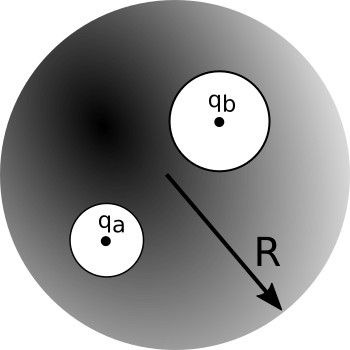
\includegraphics[width=0.5\linewidth]{./images/hw5/shielded_charges.png}
\end{figure}

\begin{enumerate}
\def\labelenumi{\arabic{enumi}.}
\tightlist
\item
  Sketch the surface charge everywhere. Explain how you know the surface
  charge looks this way.
\item
  Determine the surface charges (\(\sigma_a\), \(\sigma_b\), and
  \(\sigma_R\)).
\item
  Sketch the electric field everywhere. If the field is zero anywhere,
  indicate this explicitly. Explain how you know the electric field
  looks this way.
\item
  Determine the magnitude of electric field outside the conductor and
  inside each cavity.
\item
  If we brought an external charge \(q_c\) near the conducting sphere
  how do your answers to parts 1-4 change? You may answer in words,
  pictures or both.
\end{enumerate}

{5. Proving Uniqueness}\label{proving-uniqueness}

For this homework problem, you will prove the ``second uniqueness
theorem'' yourself, using a slightly different method than what
Griffiths does (though you may find some common ``pieces'' are
involved!) It will really help to review/read the section on the second
uniqueness theorem as you work through this problem.

\textbf{Do it like this:}

\begin{itemize}
\tightlist
\item
  Green's Identity is true for ANY choice of T and U, so let the
  functions T and U in that identity both be the SAME function.
\end{itemize}

\[\int_V \left(T \nabla^2 U + \nabla T \cdot \nabla U\right) d\tau = \oint_S \left(T \nabla U\right)\cdot d\mathbf{A}\]

\begin{itemize}
\tightlist
\item
  Specifically, you should set them both equal to \(V_3=V_1-V_2\) where
  \(V_1\) and \(V_2\) represent different solutions to the same boundary
  value problem (\(\nabla^2 V = 0\) with boundary conditions).
\item
  Then, using Green's Identity (along with some arguments about what
  happens at the boundaries, rather like Griffith's uses in his proof)
  should let you quickly show that \(E_3\), which is defined to be the
  negative gradient of \(V_3\) (as usual), must vanish everywhere
  throughout the volume. QED.
\end{itemize}

\emph{Work to understand the game. We are checking if there are two
different potential functions, \(V_1\) and \(V_2\), each of which
satisfies Laplace's equation throughout the region we're considering.
You construct (define) \(V_3\) to be the difference of these, and you
prove that \(V_3\) (or in this case, \(\mathbf{E}_3\)) must vanish
everywhere in the region. This means there really is only one unique
E-field throughout the region after all! This is another one of those
``formal manipulation'' problems, giving you a chance to practice with
the divergence theorem and think about boundary conditions.}

{6. Potential and electric field with Laplace's
equation}\label{potential-and-electric-field-with-laplaces-equation}

In class we derived the solution for the 2D version of Laplace's
equation with the boundary conditions shown below.

\begin{figure}[htbp]
\centering
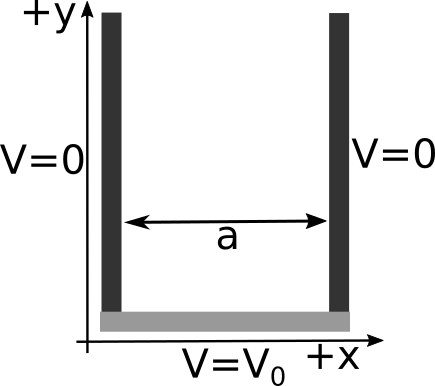
\includegraphics[width=0.5\linewidth]{./images/hw5/channel.png}
\end{figure}

That solution was analytic, but it contained an infinite series:

\[V(x,y) = \sum_{n=1,3,5,\dots}^{\infty} \dfrac{4 V_0}{\pi n} \sin \left(\dfrac{n\pi x}{a}\right)e^{-\dfrac{n\pi y}{a}}\]

While perfectly analytic, this solution is hard to visualize. What does
that solution look like? Take \(V_0 = 10V\) and \(a = 1m\).

\begin{enumerate}
\def\labelenumi{\arabic{enumi}.}
\tightlist
\item
  Plot the approximate solution in 3D space using Python's
  \texttt{mplot3D} for just the first term in the sum (i.e., only for
  \(n = 1\)). Download this
  \href{../jupyter/HW5-3dPotentialPlot.ipynb}{Jupyter notebook} (you can
  \href{https://github.com/dannycab/phy481msu/blob/gh-pages/jupyter/HW5-3dPotentialPlot.ipynb}{view
  it here}), which walks you through how to plot in 3D.
\item
  Plot the approximate solution in 3D space for the first 5 terms. What
  do you notice about the boundary where \(V=V_0\)?
\item
  Plot the approximate solution such that the boundary where \(V=V_0\)
  looks very close to constant. How many terms did you need? If you
  didn't do it for Part 2, you will have to figure out how to
  automatically compute each term to construct your plot instead of
  copying-and-pasting 50, or 100, or 1000 times!
\item
  Given this plot of the potential, sketch (by hand) what the electric
  field looks like. Recall that \(\mathbf{E} = -\nabla V\).
\end{enumerate}

{7. Potential in a cubical
box}\label{potential-in-a-cubical-box}

You have a cubical box (sides all of length \(a\)) made of 6 metal
plates that are insulated from each other. The left wall is located at
\(x=-a/2\) and the right wall is at \(x=+a/2\). Both left and right
walls are held at constant potential \(V=V_0\). All four other walls are
grounded (\(V=0\) for these walls).

(Note that we've set up the geometry so the cube runs from \(y=0\) to
\(y=a\), and from \(z=0\) to \(z=a\), but from \(x=-a/2\) to \(x=+a/2\)
This should actually make the math work out a little easier!)

\begin{enumerate}
\def\labelenumi{\arabic{enumi}.}
\tightlist
\item
  Find the potential \(V(x,y,z)\) everywhere inside the box.
\item
  Also, is V=0 at the center of this cube?
\item
  Is E=0 there? Why, or why not?
\end{enumerate}
\end{document}
